% Provenance (never printed): see sources/outline_sources.md (Year 3:
% geomorphology, hillslope processes, river incision, landscape evolution).
% Brief: sources/book5/BRIEFS.md, ch. 18. Curves from
% figdata/bachelor-3/hillslope.py, stream_profile.py and varden_river.py.
% Exercise and problem values in the Book 5 scratch calculator calc/ch18.py.
% The upland west of the Varden Hills, its river, its tributaries, its
% uplift rate and its base-level fall are invented; the outlet elevation is
% the region model's river at the west edge of the map.
\chapter{Quantitative Geomorphology}\label{ch:b3:quantitative-geomorphology}

A river crossing a rising range has a step in its long profile: a waterfall,
with a gorge below it and a gentler valley above. The step does not stay
where it formed. It climbs upstream, a few millimetres or a few metres a
year, and its position is a clock that started when the river's base was
lowered. Reading that clock, and the rates written in the shapes of hills
and rivers, takes two conservation laws and two transport laws: one for the
soil that creeps down a slope, one for the bedrock that a river cuts.

\begin{recall}
Weathering, erosion, deposition, landforms and the balance between uplift
and erosion are in the school books, as are isostatic rebound and U-shaped
glacial valleys. The denudation rate, the bed shear stress and the Shields
parameter are in the Year 1 volume, in its chapter on erosion and transport;
the digital elevation model in its chapter on geological maps; Airy
isostasy in its chapter on isostasy and gravity anomalies. \omterm{def:b3:advanced-geochronology:cosmogenic}{Cosmogenic
nuclides} and erosion rates from them are in
Chapter~\ref{ch:b3:advanced-geochronology}, \omterm{def:b3:orogenic-wedges:thermochronology}{thermochronology} and the
\omterm{def:b3:orogenic-wedges:age-elevation}{age--elevation relationship} in Chapter~\ref{ch:b3:orogenic-wedges}. The
diffusion equation is in the physics books.
\end{recall}

\section{Hillslopes}\label{sec:b3:quantitative-geomorphology:hillslopes}

On a soil-mantled hill, the soil moves downslope grain by grain: burrowing
animals throw it, roots heave it, freezing and wetting swell it, and each
disturbance lets gravity shift it a little. Averaged over centuries, the
flux of soil is proportional to the slope.

\begin{definition}[Hillslope diffusion]\label{def:b3:quantitative-geomorphology:diffusion}
\emph{Hillslope diffusion}\index{hillslope diffusion} is the slow
downslope transport of soil whose volume flux per unit width of slope,
$\vec q$, is proportional to the gradient of the surface elevation $z$:
$\vec q = -\kappa\,\nabla z$. The coefficient $\kappa$, in
\unit{m^2/yr}, is the hillslope diffusivity.
\end{definition}

\begin{theorem}[Diffusion of hillslopes]\label{thm:b3:quantitative-geomorphology:diffusion}
Let rock be uplifted at a rate $U$ relative to the channels that bound a
hillslope, soil and rock have the same density, and soil move by \omterm{def:b3:quantitative-geomorphology:diffusion}{hillslope
diffusion} with uniform $\kappa$. Then the surface elevation obeys
\[
\frac{\partial z}{\partial t} = U + \kappa\,\nabla^2 z ,
\]
the diffusion equation with a source term.
\end{theorem}

\begin{proof}
Take a small area $\delta S$ of the slope. Its volume changes by uplift,
$U\,\delta S$ per unit time, and by the soil that flows out through its
edges, $\oint \vec q\cdot\vec n\,\mathrm{d}\ell = (\nabla\cdot\vec q)\,\delta S$.
Hence $\partial z/\partial t = U - \nabla\cdot\vec q$; with $\vec q = -\kappa
\nabla z$ and $\kappa$ uniform, $\nabla\cdot\vec q = -\kappa\nabla^2 z$.
\end{proof}

A fault or a shoreline cuts a scarp at one moment; afterwards the scarp only
diffuses. Starting from a vertical step of half-height $a$ on a far-field
slope $b$, the solution in one dimension is
\[
z(x,t) = a\,\operatorname{erf}\!\left(\frac{x}{2\sqrt{\kappa t}}\right) + b\,x ,
\qquad
\left.\frac{\partial z}{\partial x}\right|_{x=0} = \frac{a}{\sqrt{\pi\kappa t}} + b .
\]
The shape depends only on the product $\kappa t$: a measured profile gives
$\kappa t$, and either an independent age gives $\kappa$, or a known
$\kappa$ gives the age, a \emph{morphological age}. Scarps in semi-arid
regions with granular soils and sparse vegetation give $\kappa$ between
$10^{-3}$ and \qty{e-2}{m^2/yr}; humid, densely vegetated coastal mountains
about \qty{5e-3}{m^2/yr}.
% ledger: whipple04:scarp-erf, whipple04:scarp-kappa

\begin{omfigure}
\begin{tikzpicture}
\begin{groupplot}[group style={group size=2 by 1, horizontal sep=1.6cm},
  width=0.48\linewidth, height=0.36\linewidth, tick label style={font=\scriptsize},
  label style={font=\small}, legend style={font=\scriptsize, draw=none, fill=none}]
\nextgroupplot[xlabel={distance $x$ (m)}, ylabel={$z$ (m)}, xmin=-40, xmax=40,
  ymin=-5, ymax=5, legend pos=north west]
% computed in figdata/bachelor-3/hillslope.py
\addplot[black!50, densely dashed] table[x=x, y=z0] {figdata/out/bachelor-3-hillslope-scarp.dat};
\addplot[omDef, thick] table[x=x, y=z1] {figdata/out/bachelor-3-hillslope-scarp.dat};
\addplot[omProp, thick] table[x=x, y=z2] {figdata/out/bachelor-3-hillslope-scarp.dat};
\addplot[omThm, thick] table[x=x, y=z3] {figdata/out/bachelor-3-hillslope-scarp.dat};
\legend{initial, \qty{2}{kyr}, \qty{10}{kyr}, \qty{40}{kyr}}
\nextgroupplot[xlabel={distance from the divide (m)}, ylabel={height (m)},
  xmin=-150, xmax=150, ymin=0, ymax=200, xtick={-150,-75,0,75,150}]
\addplot[omMeth, thick] table[x=x, y=z1] {figdata/out/bachelor-3-hillslope-hill.dat};
\addplot[omDef, thick] table[x=x, y=z2] {figdata/out/bachelor-3-hillslope-hill.dat};
\addplot[omThm, thick] table[x=x, y=z3] {figdata/out/bachelor-3-hillslope-hill.dat};
\node[font=\scriptsize, anchor=north] at (axis cs:0,45) {0.0215};
\node[font=\scriptsize, anchor=north] at (axis cs:0,94) {0.043};
\node[font=\scriptsize, anchor=north] at (axis cs:0,184) {\qty{0.086}{mm/yr}};
\end{groupplot}
\end{tikzpicture}

\par\smallskip{\small Left, a scarp of \qty{5}{m} offset on a slope of
0.05, diffusing with $\kappa = \qty{5e-3}{m^2/yr}$: the initial step
(dashed) and the profiles after 2, 10 and \qty{40}{kyr}. Right, steady
hills of half-width \qty{150}{m} with the same $\kappa$ (height above the
channels), lowering at
0.0215, 0.043 and \qty{0.086}{mm/yr}: parabolas whose relief and hilltop
curvature are proportional to the erosion rate.}\label{fig:b3:quantitative-geomorphology:hillslope}
\end{omfigure}
% ledger: whipple04:scarp-kappa

When a hill has been uplifted and eroded long enough, its shape stops
changing: every point is lowered at the rate the rock rises.

\begin{proposition}[Hilltop curvature gauges the erosion rate]\label{prop:b3:quantitative-geomorphology:curvature}
On a hillslope in \omterm{def:b3:quantitative-geomorphology:steady-profile}{steady state} under \omterm{def:b3:quantitative-geomorphology:diffusion}{hillslope diffusion}, the erosion rate
$E$, equal to $U$, is
\[
E = -\kappa\,\nabla^2 z .
\]
In one dimension the profile is the parabola $z = z_0 - E x^2/(2\kappa)$,
with relief $E L^2/(2\kappa)$ between the divide and channels a distance
$L$ away.
\end{proposition}

\begin{proof}
Setting $\partial z/\partial t = 0$ in the theorem gives $\kappa\nabla^2 z =
-U = -E$. In one dimension, two integrations with $\mathrm{d}z/\mathrm{d}x =
0$ at the divide give the parabola, and its value at $x = L$ the relief.
\end{proof}

Curvature, a geometric quantity measured on a digital elevation model, thus
reads as a rate once $\kappa$ is known: the steeper and more sharply rounded
the hilltops, the faster the landscape erodes. The soil itself is made from
the rock below at a rate that depends on how much soil already covers it.

\begin{definition}[Soil production function]\label{def:b3:quantitative-geomorphology:soil-production}
The \emph{soil production function}\index{soil production function} gives
the rate $P$ at which bedrock is converted to soil as a function of the
soil thickness $h$; it is commonly taken as $P = P_0\,e^{-h/h_0}$, where
$P_0$ is the rate on bare rock and $h_0$ a length of a fraction of a metre.
\end{definition}

At \omterm{def:b3:quantitative-geomorphology:steady-profile}{steady state} the soil-rock interface is lowered at the rate of the
surface, $P(h) = E$, so the soil thickness is $h = h_0 \ln(P_0/E)$: faster
erosion means thinner soil, and where $E$ exceeds $P_0$ the soil is
stripped and bare rock, limited by weathering, crops out. The fastest soil
production rates measured are of the order of \qty{0.5}{mm/yr}.
% ledger: whipple04:soil

Linear diffusion fails on steep slopes. As the gradient approaches a
threshold, grains roll and slide in bursts and shallow landslides strip the
soil.

\begin{definition}[Critical hillslope gradient]\label{def:b3:quantitative-geomorphology:critical}
The \emph{critical hillslope gradient}\index{critical hillslope gradient}
$S_c$ is the gradient at which the soil flux grows without bound; in a
widely used nonlinear transport law, $q = \kappa S/[1 - (S/S_c)^2]$.
\end{definition}

Slopes much gentler than $S_c$ behave as in linear diffusion; slopes that
erode fast steepen toward $S_c$ and become planar, their gradient set by the
threshold rather than by the erosion rate.
% ledger: whipple04:nonlinear

\begin{inthefield}[Scanning a hillslope]
A team surveying a soil-mantled ridge sets a terrestrial laser scanner on a
tripod a few tens of metres from the crest. Each scan records millions of
points, the distance and direction to the ground surface, through gaps in
the grass and the shrubs; the points of several scan stations are merged
into one cloud, registered to targets surveyed with a satellite receiver,
and the last returns are kept to remove the vegetation. The bare-earth cloud
is gridded into an elevation model of decimetre cells, smoothed over a few
metres, and its Laplacian computed at the crest. The team then compares the
hilltop curvatures of ridges eroding at rates measured with \omterm{def:b3:advanced-geochronology:cosmogenic}{cosmogenic
nuclides}: plotted against each other, the two give the diffusivity of the
hillslope as the slope of a line, as the proposition predicts.
\end{inthefield}

\section{River incision}\label{sec:b3:quantitative-geomorphology:rivers}

Where a river runs on bedrock, it cuts down by plucking blocks, by abrasion
under its bed load and by cavitation. All these scale with the shear stress
the flow exerts on its bed, or the power it spends there, and both grow
with discharge and slope. Discharge grows with drainage area, so area stands
for discharge.

\begin{definition}[Stream-power law]\label{def:b3:quantitative-geomorphology:stream-power}
The \emph{stream-power law}\index{stream-power law} gives the rate of
vertical incision $E$ of a bedrock river as
\[
E = K A^m S^n ,
\]
where $A$ is the drainage area upstream of the point, $S$ the channel
gradient, $m$ and $n$ positive exponents, and $K$ an erodibility
coefficient that lumps rock strength, climate and channel width.
\end{definition}

For processes that scale with shear stress or with unit stream power,
$m/n$ is close to 0.5. A survey of badland channels cut in weak rock over
about 20 years found incision rates proportional to $A^{0.44}S^{0.68}$.
% ledger: whipple04:spim

\begin{definition}[Detachment-limited and transport-limited incision]\label{def:b3:quantitative-geomorphology:limited}
Incision is \emph{detachment-limited}\index{detachment-limited incision}
when the river can carry away more sediment than it receives, so that its
rate of lowering is set by how fast it detaches bedrock from its bed: the
\omterm{def:b3:quantitative-geomorphology:stream-power}{stream-power law} applies. It is
\emph{transport-limited}\index{transport-limited incision} when the river
carries all the sediment it can, so that its bed is lowered only where the
transport capacity grows downstream, at the rate set by the divergence of
the sediment flux.
\end{definition}

A \omterm{def:b3:quantitative-geomorphology:limited}{transport-limited} river behaves much like a hillslope: the flux depends
on slope, and its profile evolves by a diffusion-like equation that rounds
off any step. A \omterm{def:b3:quantitative-geomorphology:limited}{detachment-limited} river keeps a step sharp and moves it,
as the next section shows. Mountain rivers with bedrock floors and thin
gravel are usually closer to the first; rivers on thick alluvium to the
second.

\begin{omfigure}
\begin{tikzpicture}[x=0.55cm, y=0.55cm, font=\scriptsize,
  declare function={f(\x)=2.1+3.5*(1-(\x-0.5)/10)^2;
    tl(\x,\l)=f(\x)-1.1*exp(-(10.5-\x)/\l);}]
\begin{scope}
\draw[->] (0,0) -- (11.5,0) node[below left] {distance downstream};
\draw[->] (0,0) -- (0,6) node[above right] {$z$};
\draw[black!50, densely dashed] plot[domain=0.5:10.5, samples=40] (\x,{f(\x)});
\draw[omDef, thick] plot[domain=0.5:6.5, samples=30] (\x,{f(\x)}) -- plot[domain=6.5:10.5, samples=20] (\x,{f(\x)-1.1});
\draw[omThm, thick] plot[domain=0.5:3.5, samples=20] (\x,{f(\x)}) -- plot[domain=3.5:10.5, samples=30] (\x,{f(\x)-1.1});
\draw[->, black!70] (6.3,4.1) -- (3.8,4.75);
\node[anchor=west, align=left] at (5.6,5.3) {detachment-limited:\\ the step moves upstream};
\node at (5.5,-0.7) {(a)};
\end{scope}
\begin{scope}[xshift=7.2cm]
\draw[->] (0,0) -- (11.5,0) node[below left] {distance downstream};
\draw[->] (0,0) -- (0,6) node[above right] {$z$};
\draw[black!50, densely dashed] plot[domain=0.5:10.5, samples=40] (\x,{f(\x)});
\draw[omDef, thick] plot[domain=0.5:10.5, samples=40] (\x,{tl(\x,1.2)});
\draw[omThm, thick] plot[domain=0.5:10.5, samples=40] (\x,{tl(\x,3.5)});
\node[anchor=west, align=left] at (5.0,5.3) {transport-limited:\\ the fall diffuses upstream};
\node at (5.5,-0.7) {(b)};
\end{scope}
\end{tikzpicture}

\par\smallskip{\small The response of a river to a fall of its \omterm{def:b3:quantitative-geomorphology:knickpoint}{base level}
(dashed: the profile before the fall; blue, then red: two later times),
schematic. (a) A \omterm{def:b3:quantitative-geomorphology:limited}{detachment-limited} river keeps a sharp \omterm{def:b3:quantitative-geomorphology:knickpoint}{knickpoint} that
migrates upstream; below it the profile has its old shape, lowered. (b) A
\omterm{def:b3:quantitative-geomorphology:limited}{transport-limited} river lowers its whole profile progressively, most near
the outlet.}\label{fig:b3:quantitative-geomorphology:regimes}
\end{omfigure}

If rock rises at a uniform rate $U$ relative to the river's outlet, and $K$,
$m$, $n$ are uniform, the river evolves as $\partial z/\partial t = U - K A^m
S^n$.

\begin{definition}[Steady-state river profile]\label{def:b3:quantitative-geomorphology:steady-profile}
A river profile is in \emph{steady state}\index{steady-state river profile}
when its elevation no longer changes in time: at every point incision
balances rock uplift relative to the outlet.
\end{definition}

\begin{theorem}[Steady-state profile under the stream-power law]\label{thm:b3:quantitative-geomorphology:steady}
Under uniform $U$, $K$, $m$ and $n$, a \omterm{def:b3:quantitative-geomorphology:limited}{detachment-limited} river in \omterm{def:b3:quantitative-geomorphology:steady-profile}{steady
state} has the gradient
\[
S = \left(\frac{U}{K}\right)^{1/n} A^{-m/n} .
\]
\end{theorem}

\begin{proof}
At \omterm{def:b3:quantitative-geomorphology:steady-profile}{steady state} $\partial z/\partial t = 0$, so $K A^m S^n = U$, whence $S^n
= (U/K)A^{-m}$; taking the $n$th root gives the result.
\end{proof}

\begin{omfigure}
\begin{tikzpicture}
\begin{groupplot}[group style={group size=2 by 1, horizontal sep=1.7cm},
  width=0.48\linewidth, height=0.33\linewidth, tick label style={font=\scriptsize},
  label style={font=\small}]
\nextgroupplot[xlabel={distance from the divide (km)}, ylabel={$z$ (m)},
  xmin=0, xmax=12, ymin=150, ymax=420]
% computed in figdata/bachelor-3/stream_profile.py
\addplot[omDef, thick] table[x=d, y=z] {figdata/out/bachelor-3-stream_profile-steady.dat};
\nextgroupplot[xmode=log, ymode=log, xlabel={drainage area $A$ (\unit{km^2})},
  ylabel={gradient $S$}, xmin=0.1, xmax=100, ymin=0.003, ymax=0.2]
\addplot[omDef, thick] table[x=A, y=S] {figdata/out/bachelor-3-stream_profile-steady.dat};
\addplot[only marks, mark=*, mark size=1.4pt, omThm] table[x=A, y=S] {figdata/out/bachelor-3-stream_profile-sa.dat};
\addplot[omThm, densely dashed] table[x=A, y=S] {figdata/out/bachelor-3-stream_profile-fit.dat};
\end{groupplot}
\end{tikzpicture}

\par\smallskip{\small The steady-state profile of the invented upland river
west of the Varden Hills ($U = \qty{0.043}{mm/yr}$, $K =
\qty{e-6}{yr^{-1}}$, $m = 0.5$, $n = 1$), from its channel head to the
outlet at \qty{170}{m}. Right, gradient against area: the model (blue
line) and twelve gradients measured over reaches of \qty{200}{m} with a
scatter of about \qty{10}{\percent} (red dots), whose least-squares line
(dashed) has a slope of $-0.47$.}\label{fig:b3:quantitative-geomorphology:profile}
\end{omfigure}

The gradient falls as a power of area: the profile is concave up. Real
rivers follow such a power law even when the assumptions of the theorem are
doubtful, so two numbers summarise a profile.
% ledger: whipple04:steepness

\begin{definition}[Channel steepness and concavity indices]\label{def:b3:quantitative-geomorphology:indices}
When the gradient of a river follows $S = k_s A^{-\theta}$, the exponent
$\theta$ is the \emph{concavity index}\index{concavity index} and the
coefficient $k_s$ the \emph{channel steepness index}\index{channel steepness index}.
To compare rivers, $\theta$ is set to a common reference value
$\theta_{\mathrm{ref}}$, and $k_{sn} = S A^{\theta_{\mathrm{ref}}}$ is the
normalised steepness.
\end{definition}

By the theorem, $\theta = m/n$ and $k_s = (U/K)^{1/n}$: at a given
erodibility, a river is steeper where rock rises faster. Steepness maps of
a range therefore outline its uplift.


Gradients are derivatives of noisy elevations and scatter widely. Integrating
the profile instead uses elevations, which are better measured.

\begin{definition}[Chi analysis]\label{def:b3:quantitative-geomorphology:chi}
\emph{Chi analysis}\index{chi analysis} plots the elevation of the points
of a river network against the coordinate
\[
\chi(x) = \int_{x_b}^{x} \left(\frac{A_0}{A(x')}\right)^{\theta}
\mathrm{d}x' ,
\]
where $x$ is the distance upstream along the channel from a base point
$x_b$, $A_0$ a reference area and $\theta$ the \omterm{def:b3:quantitative-geomorphology:indices}{concavity index}; $\chi$ has
the dimension of a length.
\end{definition}

\begin{proposition}[The chi transform straightens a steady profile]\label{prop:b3:quantitative-geomorphology:chi}
Under the assumptions of the steady-state theorem, with $\theta = m/n$,
every channel of a network draining to the base elevation $z_b$ satisfies
\[
z = z_b + \left(\frac{U}{K A_0^{m}}\right)^{1/n} \chi :
\]
all channels lie on one straight line of slope $k_s A_0^{-\theta}$ in the
$(\chi, z)$ plane.
\end{proposition}

\begin{proof}
Along a channel, $\mathrm{d}z/\mathrm{d}x = S = k_s A^{-\theta} = k_s
A_0^{-\theta}(A_0/A)^{\theta}$. Integrating from $x_b$, where $z = z_b$,
gives $z = z_b + k_s A_0^{-\theta}\chi$, and $k_s A_0^{-\theta} =
(U/K)^{1/n} A_0^{-m/n}$. A tributary joins the trunk at a junction whose
$z$ and $\chi$ it shares, and obeys the same relation upstream of it.
\end{proof}

A channel that departs from the line is not in \omterm{def:b3:quantitative-geomorphology:steady-profile}{steady state}, or crosses
rock of a different erodibility, or has lost or captured drainage area: a
tributary that plots above its neighbours at the same $\chi$ is being
robbed of area, one that plots below is growing.

\section{Transient landscapes}\label{sec:b3:quantitative-geomorphology:transient}

\begin{definition}[Base level and knickpoint]\label{def:b3:quantitative-geomorphology:knickpoint}
The \emph{base level}\index{base level} of a river is the elevation of its
outlet, below which it cannot cut: the sea, a lake, or the trunk river it
joins. A \emph{knickpoint}\index{knickpoint} is a place where the gradient
of a river's long profile increases abruptly, from a steepened reach to a
waterfall.
\end{definition}

A \omterm{def:b3:quantitative-geomorphology:knickpoint}{knickpoint} may be fixed, where the river crosses a harder bed or a fault
scarp that is still active, or mobile, where it is the head of the
river's response to a change below it: a fall of \omterm{def:b3:quantitative-geomorphology:knickpoint}{base level}, a faster
uplift.
% ledger: whipple04:response

\begin{theorem}[Knickpoints as kinematic waves]\label{thm:b3:quantitative-geomorphology:kinematic}
Let $n = 1$, with $U$, $K$ and $m$ uniform, and let $x$ be the distance
upstream from the outlet. Then $z$ obeys
\[
\frac{\partial z}{\partial t} + K A^m \frac{\partial z}{\partial x} = U ,
\]
and any feature of the profile, a step included, travels upstream at the
celerity $c = K A^m$ while keeping its height. A \omterm{def:b3:quantitative-geomorphology:knickpoint}{knickpoint} starting at
the outlet at $t = 0$ reaches the point $x$ at the time
\[
t(x) = \int_0^x \frac{\mathrm{d}x'}{K A(x')^m} = \frac{\chi(x)}{K A_0^m},
\]
with $\chi$ computed with $\theta = m$. All the \omterm{def:b3:quantitative-geomorphology:knickpoint}{knickpoints} born in a network
at the same time therefore lie at the same $\chi$, and on the same contour.
\end{theorem}

\begin{proof}
With $x$ upstream, the gradient is $S = \partial z/\partial x$, and the
evolution equation $\partial z/\partial t = U - K A^m S$ is the equation
written. Along a curve $\mathrm{d}x/\mathrm{d}t = K A(x)^m$, its left side
is the total derivative $\mathrm{d}z/\mathrm{d}t$, so $z$ grows by $U$ per
unit time along every such curve. Two points on either side of a step,
carried along neighbouring curves, gain the same height, so the step keeps
its height and moves with the curves. The time to reach $x$ is
$\int \mathrm{d}x'/c$, which is $\chi(x)/(K A_0^m)$ by the definition of
$\chi$ with $\theta = m$. In the network, $\chi$ is measured along each
flow path from the same outlet, so equal times mean equal $\chi$, and by
the proposition on $\chi$ the reaches below the \omterm{def:b3:quantitative-geomorphology:knickpoint}{knickpoints}, already
adjusted to the new \omterm{def:b3:quantitative-geomorphology:knickpoint}{base level}, put them all at the same elevation.
\end{proof}

The celerity grows with drainage area: a \omterm{def:b3:quantitative-geomorphology:knickpoint}{knickpoint} runs fast through the
trunk and slows in the headwaters. The time it takes to cross the whole
network to the channel heads is the \emph{response time} of the landscape,
of the order of a million years for typical uplift rates. When $n \ne 1$
the celerity also depends on the slope, and a step changes shape: for $n >
1$ its steep face outruns the reaches around it and stays sharp, for $n <
1$ it lags and spreads.

\begin{omfigure}
\begin{tikzpicture}
\begin{groupplot}[group style={group size=2 by 1, horizontal sep=1.5cm},
  width=0.5\linewidth, height=0.42\linewidth, tick label style={font=\scriptsize},
  label style={font=\small}, legend style={font=\scriptsize, draw=none, fill=none}]
\nextgroupplot[xlabel={distance from the divide (km)}, ylabel={$z$ (m)}, xmin=0, xmax=12.2,
  ymin=160, ymax=440, legend pos=north east]
% computed in figdata/bachelor-3/stream_profile.py
\addplot[black!50, densely dashed] table[x=d, y=z0] {figdata/out/bachelor-3-stream_profile-knick.dat};
\addplot[omMeth, thick] table[x=d, y=z1] {figdata/out/bachelor-3-stream_profile-knick.dat};
\addplot[omDef, thick] table[x=d, y=z2] {figdata/out/bachelor-3-stream_profile-knick.dat};
\addplot[omThm, thick] table[x=d, y=z3] {figdata/out/bachelor-3-stream_profile-knick.dat};
\legend{before, \qty{300}{kyr}, \qty{600}{kyr}, \qty{900}{kyr}}
\nextgroupplot[xlabel={$\chi$ (m)}, ylabel={$z$ (m)}, xmin=0, xmax=7500, ymin=160, ymax=520,
  scaled x ticks=false, xtick={0,2000,4000,6000}, xticklabels={0,2000,4000,6000},
  legend pos=north west]
% computed in figdata/bachelor-3/varden_river.py
\addplot[black!35, line width=2.2pt] table[x=chi, y=z] {figdata/out/bachelor-3-varden_river-trunk.dat};
\addplot[omMeth, only marks, mark=o, mark size=1.3pt, each nth point=8] table[x=chi, y=z] {figdata/out/bachelor-3-varden_river-trib1.dat};
\addplot[omDef, only marks, mark=square, mark size=1.2pt, each nth point=8] table[x=chi, y=z] {figdata/out/bachelor-3-varden_river-trib2.dat};
\addplot[omProp, only marks, mark=diamond, mark size=1.5pt, each nth point=8] table[x=chi, y=z] {figdata/out/bachelor-3-varden_river-trib3.dat};
\addplot[black, densely dashed, domain=0:7500, samples=2] {170 + 0.043*x};
\addplot[only marks, mark=triangle*, mark size=2.8pt, omThm] table[x=chi, y=zhi] {figdata/out/bachelor-3-varden_river-knicks.dat};
\legend{trunk, trib.~1, trib.~2, trib.~3, steady}
\end{groupplot}
\end{tikzpicture}

\par\smallskip{\small Left, the upland river after a fall of \qty{25}{m} of
its \omterm{def:b3:quantitative-geomorphology:knickpoint}{base level} ($n = 1$): the \omterm{def:b3:quantitative-geomorphology:knickpoint}{knickpoint}, a waterfall of constant height,
reaches 1.7, 3.3 and \qty{4.6}{km} above the outlet after 300, 600 and
\qty{900}{kyr}; below it the river has the old shape, \qty{25}{m} lower.
Right, chi plot ($A_0 = \qty{1}{km^2}$, $\theta = 0.5$) of the trunk and
three tributaries at \qty{900}{kyr}: below $\chi = \qty{900}{m}$ every
channel lies on the steady-state line through the outlet (dashed), above it
on the old line, \qty{25}{m} higher. The waterfalls of the trunk and of
tributary 3 sit at the same $\chi$ (red triangle); tributaries 1 and 2 join
the trunk above it and have not yet been
reached.}\label{fig:b3:quantitative-geomorphology:knick}
\end{omfigure}

\begin{inthefield}[A waterfall that walks upstream]
\begin{minipage}[t]{0.40\linewidth}\vspace{0pt}
At Niagara the river drops into a gorge it has cut itself. About
\num{12500} years ago the Falls stood at the edge of the Niagara
Escarpment; since then, as the water wore away the rocks of the escarpment
and blocks broke from the crest, the crest has moved about \qty{11}{km}
upstream: about a metre a year on average, about a tenth of that today.
Erosion is slower when the crest is a long horseshoe that spreads the
water. The gorge is the path of the \omterm{def:b3:quantitative-geomorphology:knickpoint}{knickpoint}.
\end{minipage}\hfill
\begin{minipage}[t]{0.56\linewidth}\vspace{0pt}
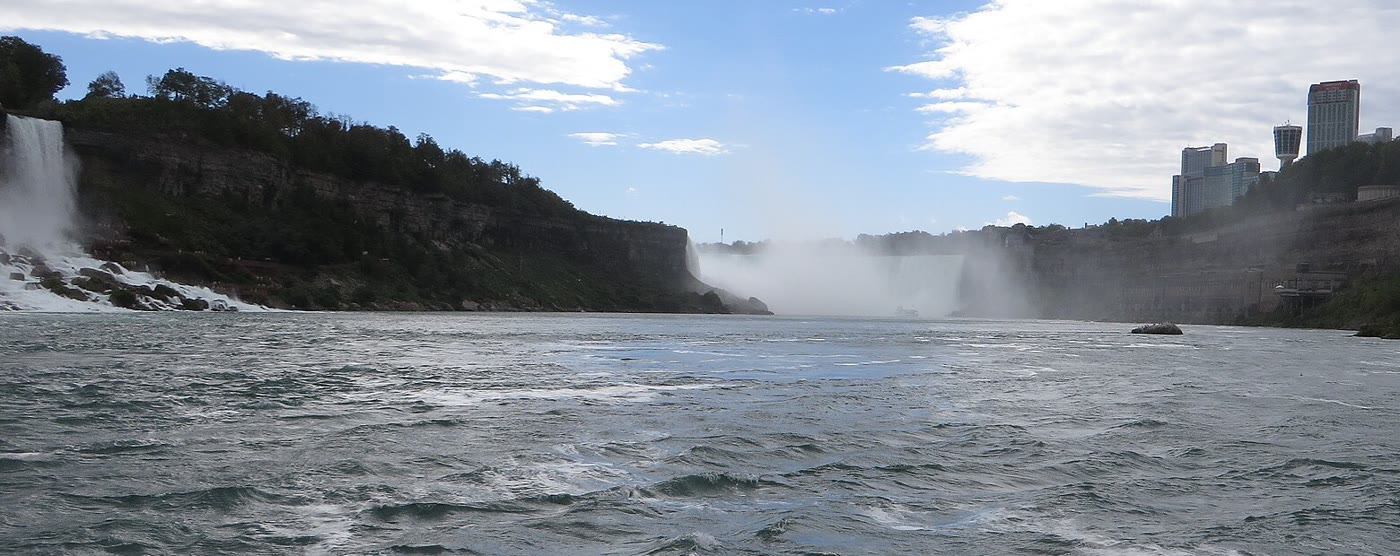
\includegraphics[width=\linewidth]{images/book5/b3-niagara-gorge.jpg}

{\scriptsize The Niagara Gorge, looking upstream to the Horseshoe Falls in
their mist, the American Falls at the left edge. Photo Ken Lund,
CC BY-SA 2.0 (cropped).}
\end{minipage}
\end{inthefield}
% ledger: ijc18:niagara, photo:b3-niagara-gorge


\section{Glacial erosion}\label{sec:b3:quantitative-geomorphology:glacial}

A glacier sliding over its bed (basal sliding,
Chapter~\ref{ch:b3:glaciology}) erodes it by abrasion, as debris held in
the ice scours the rock, and by quarrying, as it pulls out blocks loosened
by cracks. Both scale with the speed of sliding.

\begin{definition}[Glacial erosion law]\label{def:b3:quantitative-geomorphology:glacial}
A \emph{glacial erosion law}\index{glacial erosion law} gives the rate of
erosion of a glacier's bed as $E = K_G\,u_s^{\,l}$, where $u_s$ is the
sliding speed, $K_G$ a coefficient and $l$ an exponent.
\end{definition}

Landscape models usually take $l = 1$, with values between 1 and 2 in use.
A compilation of 38 glaciers, whose erosion rates span five orders of
magnitude, found erosion correlated with sliding speed, with $l = 0.65$ and
$K_G = 10^{-4}$ for $E$ in metres a year: erosion is fastest under temperate
glaciers fed by abundant snow, which slide fast. Since the ice is thickest
and fastest along the axis of a valley, the floor is deepened more than the
sides and the valley takes its U shape.
% ledger: cook20:glacial

\begin{definition}[Glacial buzzsaw]\label{def:b3:quantitative-geomorphology:buzzsaw}
The \emph{glacial buzzsaw}\index{glacial buzzsaw} is the limit set on the
height of a mountain range by glaciers: where rock rises above the altitude
at which glaciers form, they erode it as fast as it rises, whatever the
uplift rate, so that peaks and mean elevation cluster near that altitude.
\end{definition}

\section{Tectonics and erosion}\label{sec:b3:quantitative-geomorphology:tectonics}

\begin{definition}[Topographic steady state]\label{def:b3:quantitative-geomorphology:steady-state}
A landscape is in \emph{topographic steady state}\index{topographic steady state}
when its erosion rate equals the rock uplift rate everywhere, so
that its elevations do not change though rock passes through it.
\end{definition}

Rates measured over different spans of time test the state. \omterm{def:b3:advanced-geochronology:cosmogenic}{Cosmogenic
nuclides} in river sand give the mean erosion rate of a basin over the time
needed to remove a layer of the order of the attenuation length of their
production, some \qty{55}{cm} of rock; \omterm{def:b3:orogenic-wedges:thermochronology}{thermochronometers} and their \omterm{def:b3:orogenic-wedges:age-elevation}{age--elevation relationships} give the
exhumation rate over millions of years. Where the two agree with each other
and with the uplift rate, the landscape is likely in \omterm{def:b3:quantitative-geomorphology:steady-profile}{steady state}; where
the short-term rate is faster in the lower reaches than in the headwaters,
a \omterm{def:b3:quantitative-geomorphology:knickpoint}{knickpoint} is passing through. Removing rock also unloads the
lithosphere, which rises in response.
% ledger: zech04:exposure

\begin{definition}[Erosional isostatic rebound]\label{def:b3:quantitative-geomorphology:rebound}
\emph{Erosional isostatic rebound}\index{erosional isostatic rebound} is
the rise of the rock surface of a region in isostatic equilibrium in
response to the mass removed by erosion.
\end{definition}

\begin{proposition}[Peaks rise as valleys deepen]\label{prop:b3:quantitative-geomorphology:rebound}
In Airy isostasy with crust of density $\rho_c$ over mantle of density
$\rho_m$, removing a mean thickness $\bar e$ of crust from a region raises
the whole region by $(\rho_c/\rho_m)\,\bar e$. If the erosion is confined
to the valleys, the uneroded summits rise by that amount, while the mean
surface falls by only $(1 - \rho_c/\rho_m)\,\bar e$.
\end{proposition}

\begin{proof}
Compensation requires the mass of every column above a fixed depth to stay
the same. Removing a thickness $\bar e$ of crust, averaged over the area
of compensation, lowers the mass per unit area by $\rho_c \bar e$;
replacing it requires mantle to flow in at depth, raising the base of the
column, and everything on it, by $\delta$ with $\rho_m \delta = \rho_c \bar
e$. A summit that lost no rock rises by $\delta$; the mean surface loses
$\bar e$ and gains $\delta$.
\end{proof}

The thickness-weighted density of the crust of the reference Earth model is
\qty{2.72}{g/cm^3} and that of the mantle below its Moho \qty{3.38}{g/cm^3},
a ratio of 0.80: of every hundred metres of rock eroded, the mean surface
loses only twenty. Deep incision of an old plateau can thus raise its
summits even as the plateau wears down.
% ledger: prem:crust-mantle-ratio

\begin{omfigure}
\begin{tikzpicture}[x=0.6cm, y=0.6cm, font=\scriptsize]
\begin{scope}
\fill[omDef!12] (0,0) rectangle (8,4);
\draw[thick] (0,4) -- (8,4);
\draw[densely dashed] (0,0) -- (8,0);
\node[anchor=north] at (4,-0.1) {base of the crust};
\node at (4,2) {crust $\rho_c$};
\node at (4,-1.2) {mantle $\rho_m$};
\node[anchor=south] at (4,4.1) {before};
\end{scope}
\begin{scope}[xshift=6.2cm]
\fill[omDef!12] (0,0.8) -- (0,4.8) -- (1.4,4.8) -- (2.0,2.4) -- (2.6,4.8) -- (5.4,4.8) -- (6.0,2.4) -- (6.6,4.8) -- (8,4.8) -- (8,0.8) -- cycle;
\draw[thick] (0,4.8) -- (1.4,4.8) -- (2.0,2.4) -- (2.6,4.8) -- (5.4,4.8) -- (6.0,2.4) -- (6.6,4.8) -- (8,4.8);
\draw[black!50, densely dashed] (0,4) -- (8,4);
\draw[densely dashed] (0,0.8) -- (8,0.8);
\draw[densely dashed, black!40] (0,0) -- (8,0);
\draw[<->, omThm] (8.3,4.05) -- (8.3,4.75) node[midway, right] {$\delta$};
\draw[<->, omThm] (8.3,0.05) -- (8.3,0.75) node[midway, right] {$\delta$};
\node[anchor=west, font=\scriptsize] at (8.1,2.4) {$\delta = (\rho_c/\rho_m)\,\bar e$};
\node[anchor=south] at (4,5.0) {after incision of the valleys};
\node[anchor=north] at (2.0,2.3) {valley};
\end{scope}
\end{tikzpicture}

\par\smallskip{\small \omterm{def:b3:quantitative-geomorphology:rebound}{Erosional isostatic rebound}, schematic. Cutting
valleys removes a mean thickness $\bar e$ of crust; the column rises by
$\delta = (\rho_c/\rho_m)\bar e$ at its base and at its untouched summits
(the grey dashed line is the old surface).}\label{fig:b3:quantitative-geomorphology:rebound}
\end{omfigure}

\section{Exercises}

\begin{exercise}[$\star$]\label{exo:b3:quantitative-geomorphology:1}
A shoreline scarp of offset \qty{4}{m} ($a = \qty{2}{m}$) stands on a
far-field slope of 0.04, and its steepest gradient is now 0.30. Compute
$\kappa t$, then the age of the scarp with $\kappa = \qty{5e-3}{m^2/yr}$.
\end{exercise}
% ledger: whipple04:scarp-erf, whipple04:scarp-kappa

\begin{exercise}[$\star$]\label{exo:b3:quantitative-geomorphology:2}
A lidar survey gives a hilltop curvature of \qty{-0.012}{m^{-1}} on a ridge
of diffusivity \qty{4e-3}{m^2/yr}. Compute its erosion rate in
\unit{mm/yr}, and the relief between its crest and channels
\qty{80}{m} away, assuming \omterm{def:b3:quantitative-geomorphology:steady-profile}{steady state}.
\end{exercise}

\begin{exercise}[$\star$]\label{exo:b3:quantitative-geomorphology:3}
With $m = 0.5$, $n = 1$ and $K = \qty{2e-6}{yr^{-1}}$, compute the
incision rate of a river draining \qty{25}{km^2} on a gradient of 0.01.
What are the units of $K$ for general $m$ and $n$?
\end{exercise}

\begin{exercise}[$\star$]\label{exo:b3:quantitative-geomorphology:4}
Three rivers show \omterm{def:b3:quantitative-geomorphology:knickpoint}{knickpoints}: (a) where a sandstone bed crosses a valley
cut in shale; (b) where a river crosses an active normal fault from the
footwall to the hanging wall; (c) in every river of a basin, all at about
the same elevation, a few kilometres above a coast that rose in an
earthquake. Which are fixed and which will migrate?
\end{exercise}

\begin{exercise}[$\star\star$]\label{exo:b3:quantitative-geomorphology:5}
For $m = 1$ and $n = 2$, compute $\theta$ and the steady gradient where $A =
\qty{10}{km^2}$, with $U = \qty{0.1}{mm/yr}$ and $K = 10^{-9}$ in metres and
years.
By what factor does the steepness change if $U$ doubles? Compare with $n =
1$.
\end{exercise}

\begin{exercise}[$\star\star$]\label{exo:b3:quantitative-geomorphology:6}
A river's drainage area grows with the distance $d$ from its divide as $A =
c\,d^{h}$. Show that, measured upstream from its outlet at $d = L$,
\[
\chi(d) = \frac{A_0^{\theta}}{c^{\theta}}\,\frac{L^{p} - d^{p}}{p},
\qquad p = 1 - h\theta ,
\]
and compute it for $c = 2$ (SI), $h = 1.8$, $\theta = 0.45$, $A_0 =
\qty{1}{km^2}$, $L = \qty{20}{km}$ and $d = \qty{5}{km}$.
\end{exercise}

\begin{exercise}[$\star\star$]\label{exo:b3:quantitative-geomorphology:7}
With $n = 1$, $m = 0.5$ and $K = \qty{2e-6}{yr^{-1}}$, compute the
celerity of a \omterm{def:b3:quantitative-geomorphology:knickpoint}{knickpoint} where $A = \qty{100}{km^2}$, in m/kyr, and the
time it would take to travel \qty{5}{km} at that speed. Why does it
actually take longer?
\end{exercise}

\begin{exercise}[$\star\star$]\label{exo:b3:quantitative-geomorphology:8}
Valleys \qty{600}{m} deep, occupying on average \qty{40}{\percent} of the
area of a plateau, are cut into it. With $\rho_c/\rho_m = 0.80$, compute
the mean thickness eroded, the rise of the summits and the change of the
mean elevation.
\end{exercise}
% ledger: prem:crust-mantle-ratio

\begin{exercise}[$\star\star$]\label{exo:b3:quantitative-geomorphology:9}
A \omterm{def:b3:quantitative-geomorphology:soil-production}{soil production function} has $P_0 = \qty{0.3}{mm/yr}$ and $h_0 =
\qty{0.5}{m}$. Compute the steady soil thickness for erosion at
\qty{0.05}{mm/yr} and at \qty{0.2}{mm/yr}. What happens at
\qty{0.4}{mm/yr}?
\end{exercise}

\begin{exercise}[$\star\star\star$]\label{exo:b3:quantitative-geomorphology:10}
A hill in \omterm{def:b3:quantitative-geomorphology:steady-profile}{steady state} erodes at $E = \qty{0.1}{mm/yr}$ with $\kappa =
\qty{5e-3}{m^2/yr}$ and the nonlinear law of the critical gradient, taking
$S_c = 1.2$ for the exercise. Show that the flux at a distance $x$ from the
divide is $E x$, solve for the gradient, and compute it at 20, 50, 100 and
\qty{200}{m}. Compare with linear diffusion and describe the shape of the
hill.
\end{exercise}

\begin{exercise}[$\star\star\star$]\label{exo:b3:quantitative-geomorphology:11}
Show that the response time of a river network to a change at its outlet,
for $n = 1$, is $\chi_h/(K A_0^m)$, where $\chi_h$ is the largest value of
$\chi$ at a channel head. Compute it for the upland river of the figures
($A_0 = \qty{1}{km^2}$, $m = 0.5$, $K = \qty{e-6}{yr^{-1}}$), first for its
trunk alone, whose head is at $\chi = \qty{5464}{m}$, then for the network,
whose highest head, on tributary 1, is at $\chi = \qty{7237}{m}$.
\end{exercise}

\begin{exercise}[$\star\star\star$]\label{exo:b3:quantitative-geomorphology:12}
In a network with $n = 1$ and uniform $U$, one tributary flows on rock twice
as erodible as the rest ($2K$) above its junction, at $\chi_j$. Show that
its steady-state line in the $(\chi, z)$ plane has half the slope of the
trunk's above $\chi_j$, and that a \omterm{def:b3:quantitative-geomorphology:knickpoint}{knickpoint} born at the outlet reaches,
at the time when the trunk's \omterm{def:b3:quantitative-geomorphology:knickpoint}{knickpoint} is at $\chi_k > \chi_j$, the point
of $\chi = \chi_j + 2(\chi_k - \chi_j)$ of that tributary.
\end{exercise}

\section{Problem: The Waterfall of the Varden River}

\begin{problem}[{Weekend problem --- the profile, steepness and erodibility
of an invented upland river, and the age of its waterfall}]
\label{pb:b3:quantitative-geomorphology:1}
West of the Varden Hills, the river drains an upland of schist before it
enters the map at its west edge, at an elevation of \qty{170}{m}. Upstream
of that point, its outlet, the trunk is \qty{12}{km} long from its divide,
with a drainage area $A = 4.5\,d^{1.7}$ (\unit{m^2}, $d$ in metres from the
divide) and a channel head at $d = \qty{300}{m}$. Take as the rate of rock
uplift the denudation rate of the Varden river's basin found from its loads
in the Year 1 volume, \qty{43}{m/Myr}. Take $n = 1$ and the reference area $A_0 = \qty{1}{km^2}$.
A waterfall \qty{25}{m} high stands on the trunk \qty{4.60}{km} upstream of
the outlet. All values are invented.

\medskip\noindent\textbf{Part I --- The profile.}
\begin{enumerate}
\item Compute the drainage area at the outlet and at the channel head.
\item Gradients measured over reaches of \qty{200}{m}, away from the
  waterfall:

  \smallskip
  {\small\begin{tabular}{l*{6}{c}}
  $A$ (\unit{km^2}) & 0.388 & 0.587 & 0.888 & 1.345 & 2.036 & 3.082 \\
  $S$ & 0.06641 & 0.05026 & 0.04888 & 0.03322 & 0.03688 & 0.02688 \\[2pt]
  $A$ (\unit{km^2}) & 4.665 & 7.061 & 10.69 & 16.18 & 24.49 & 37.08 \\
  $S$ & 0.01921 & 0.01713 & 0.01545 & 0.01419 & 0.007922 & 0.007855
  \end{tabular}}

  \smallskip
  Estimate the \omterm{def:b3:quantitative-geomorphology:indices}{concavity index} from the first and last points.
\item The least-squares slope of $\log S$ against $\log A$ is $-0.466$.
  Is it consistent with $\theta = 0.5$?
\item With $\theta_{\mathrm{ref}} = 0.5$, compute $k_{sn} = S A^{0.5}$ ($A$ in
  \unit{m^2}) for the first and the last point, and say what the geometric
  mean of the twelve values, \qty{45.1}{m}, represents.
\item Why do gradients scatter so much more than elevations?
\item Using the formula of the chi exercise, compute $\chi$ at $d =
  \qty{9.00}{km}$, a point below the waterfall.
\end{enumerate}

\medskip\noindent\textbf{Part II --- Steepness and erodibility.}
\begin{enumerate}[resume]
\item The river is at \qty{193.4}{m} at $d = \qty{9.00}{km}$. Compute the
  slope of the chi plot below the waterfall and the steepness $k_{sn}$.
\item Which estimate of $k_{sn}$, this one or the slope-area one, would you
  trust, and why?
\item Assuming \omterm{def:b3:quantitative-geomorphology:steady-profile}{steady state} below the waterfall, compute $K$ from the
  uplift rate.
\item Check that the incision rate at the outlet, whose gradient is
  0.00691, equals the uplift rate.
\item Compute the celerity of a \omterm{def:b3:quantitative-geomorphology:knickpoint}{knickpoint} at the outlet and at the
  waterfall, in m/kyr.
\item Compute the elevation of the channel head on the steady profile, and
  the relief of the trunk.
\end{enumerate}

\medskip\noindent\textbf{Part III --- The waterfall.}
\begin{enumerate}[resume]
\item Why, with $n = 1$, has the waterfall kept the height of the fall of
  \omterm{def:b3:quantitative-geomorphology:knickpoint}{base level}?
\item Compute $\chi$ at the waterfall.
\item Compute the time the \omterm{def:b3:quantitative-geomorphology:knickpoint}{knickpoint} took from the outlet to its present
  place.
\item Where will it be \qty{300}{kyr} from now?
\item Tributary 3 joins the trunk \qty{2.5}{km} upstream of the outlet; it
  is \qty{5}{km} long, with $A = 1.5\,s^{1.7}$ ($s$ from its own divide).
  Where should its waterfall be?
\item Tributaries 1 and 2 join the trunk 8 and \qty{5}{km} upstream of the
  outlet. Explain why they have no waterfall.
\end{enumerate}

\medskip\noindent\textbf{Part IV --- The hillslopes and the age.}
\begin{enumerate}[resume]
\item A lidar survey above the waterfall gives a hilltop curvature of
  \qty{-0.0086}{m^{-1}}. With $\kappa = \qty{5e-3}{m^2/yr}$, compute the
  erosion rate and compare it with the uplift rate.
\item The hillslopes are about \qty{150}{m} long. Compare their response
  time $L^2/\kappa$ with the age found in Part III.
\item Describe the hillslopes below the waterfall today, and how they will
  change.
\item The uplift rate is known to \qty{20}{\percent}. Give the range of the
  age.
\item How would the waterfall have evolved if $n$ were 2?
\item Give the age of the fall of \omterm{def:b3:quantitative-geomorphology:knickpoint}{base level}.
\end{enumerate}
\end{problem}
% ledger: whipple04:steepness, whipple04:scarp-kappa
